\documentclass[10pt,aspectratio=169]{beamer}
\usepackage{wmtheme}
\usepackage{multicol}

\title{Control Flow Reconstruction: AMD RDNA3 Wavefront Divergence Lifting}
\author{Christian Benjamin, Takashi Idobe}

\begin{document}

    \begin{frame}[plain]
        \titlepage
    \end{frame}
	
    \begin{frame}{Introduction}
        \begin{multicols}{2} 
                \begin{itemize}
                    \item How do GPUs execute code? \\
                        {\color{darkgray} \scriptsize{GPUs use a very different pipeline than the CPU super-scalar design}}
                    \item How do GPUs handle control flow? \\
                        {\color{darkgray} \scriptsize{Control flow is dispatched in batches (i.e. masked groups of threads)}}
                    \item What is Divergence? \\
                        {\color{darkgray} \scriptsize{Active vs inactive threads as a result of control flow branching}}
                    \item What is a lifter/IR? \\
                        {\color{darkgray} \scriptsize{Reverse engineering tool to bring compiled binaries up to a human-readable
                        Intermediate Representation layer (such as LLVM)}}
                \end{itemize}
                \begin{figure}[H]
                    \centering
                    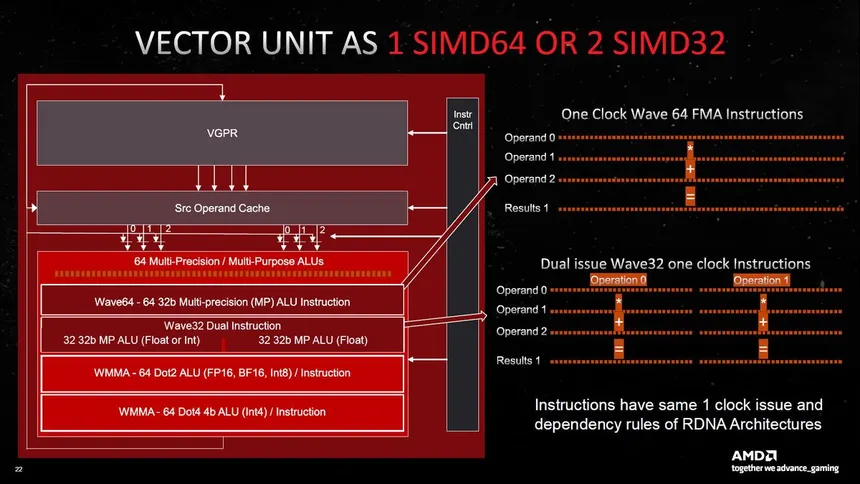
\includegraphics[width=0.75\linewidth]{images/gpu-pipeline.png}
                    \label{fig:images/gpu-pipeline.png}
                \end{figure}
                \begin{figure}[H]
                    \centering
                    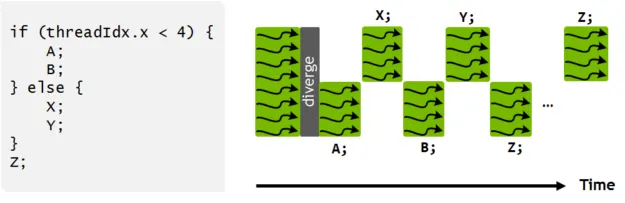
\includegraphics[width=0.75\linewidth]{images/divergence.png}
                    \label{fig:images/divergence.png}
                \end{figure}
        \end{multicols}
	\end{frame}

    \begin{frame}{Background: CPU Pipeline}
        \begin{itemize}
            \item The CPU Super Scalar Pipeline allows for forwarding, branch prediction, and (fairly) clear control flow
            \item Control flow can execute Out Of Order (OOO), but it is still deterministic
            \item Branch prediction is a natural optimization, but can come with a heavy cost if wrong
        \end{itemize}
        \begin{figure}[H]
            \centering
            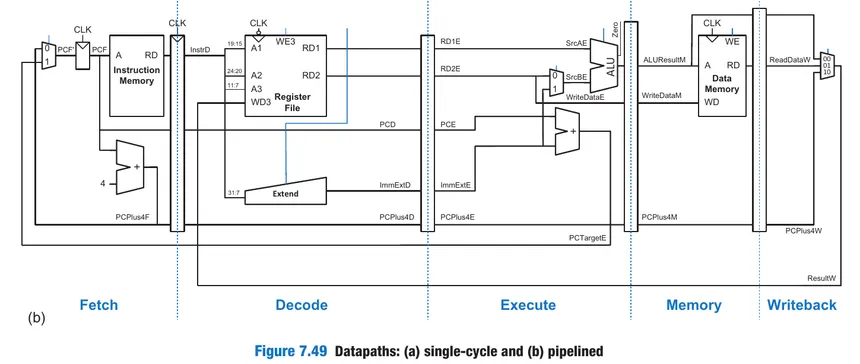
\includegraphics[width=0.5\linewidth]{images/cpu_pipeline.png}
            \label{fig:images/cpu_pipeline.png}
            \caption{CPU Pipeline}
        \end{figure}
	\end{frame}

    \begin{frame}{Background: GPU Pipeline}
        \begin{itemize}
            \item GPU pipeline is more restrictive: there is no OOO processing, or branch prediction
            \item GPU SIMT execution still allows for pipeline parallelism (forwarding)
            \item Control flow is far more difficult, and introduces heavy potential costs
        \end{itemize}

        \begin{figure}[H]
            \centering
            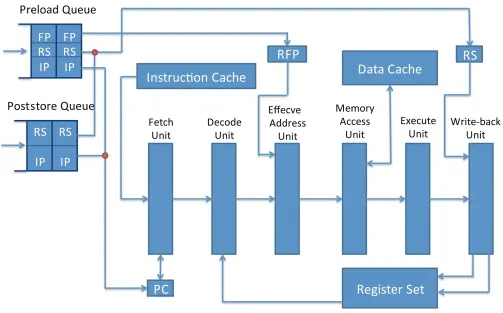
\includegraphics[width=0.5\linewidth]{images/amd_pipeline.png}
            \label{fig:images/amd_pipeline.png}
            \caption{GPU Pipeline}
        \end{figure}
	\end{frame}

    \begin{frame}{Motivation}
        \begin{itemize}
            \item Divergence comes at a heavy cost

        \end{itemize}
	\end{frame}

    \begin{frame}{Design}
        
    \end{frame}


    \begin{frame}{Implementation}

	\end{frame}


    \begin{frame}{Evaluation}

	\end{frame}


    \begin{frame}{Evalutation 2}

	\end{frame}


    \begin{frame}{Discussion}


	\end{frame}


    \begin{frame}{Limitations}

	\end{frame}

     \begin{frame}{Conclusion}

	\end{frame}

\end{document}
